\documentclass[aspectratio=169,11pt]{beamer}
\usepackage[T1]{fontenc}
\usepackage{lmodern,amsmath,amssymb,mathtools,bm,booktabs,array,graphicx,tikz}
\usetikzlibrary{arrows.meta,positioning,calc,decorations.pathreplacing,patterns}
\definecolor{ink}{HTML}{17344D}\definecolor{accent}{HTML}{087E8B}\definecolor{pale}{HTML}{EDF5F5}\definecolor{gold}{HTML}{AD6B19}
\providecommand{\dd}{\,\mathrm{d}}\providecommand{\R}{\mathbb{R}}
\providecommand{\E}{\mathbb{E}}\providecommand{\Var}{\operatorname{Var}}
\providecommand{\Cov}{\operatorname{Cov}}\providecommand{\diag}{\operatorname{diag}}
\providecommand{\norm}[1]{\left\lVert#1\right\rVert}
\providecommand{\abs}[1]{\left|#1\right|}
\usefonttheme{professionalfonts}
\setbeamercolor{normal text}{fg=black,bg=white}
\setbeamercolor{frametitle}{fg=ink,bg=white}
\setbeamercolor{title}{fg=ink}\setbeamercolor{structure}{fg=accent}
\setbeamercolor{block title}{fg=ink,bg=pale}\setbeamercolor{block body}{fg=black,bg=pale!40}
\setbeamercolor{alerted text}{fg=accent}
\setbeamerfont{frametitle}{size=\Large,series=\bfseries}
\setbeamerfont{title}{size=\LARGE,series=\bfseries}
\setbeamertemplate{navigation symbols}{}
\setbeamersize{text margin left=.7cm,text margin right=.7cm}
\setbeamertemplate{frametitle}{\vspace{.18cm}\insertframetitle\par\vspace{.1cm}{\color{accent}\hrule height .6pt}\vspace{.12cm}}
\newcommand{\notestarget}{notes.pdf}\newcommand{\noteslabel}{Notes}
\setbeamertemplate{footline}{\hspace{.7cm}\color{ink}\scriptsize Scientific Computing in Python / 2027\quad\href{\notestarget}{\noteslabel}\hfill\insertframenumber\,/\,\inserttotalframenumber\hspace{.7cm}\vspace{.18cm}}
\setbeamercovered{invisible}
\hypersetup{pdfauthor={Zan Ahmad},pdftitle={Linear observations and a two-compartment exchange model},pdfpagemode=UseNone}
\begin{document}
\begin{frame}[plain]\vfill
{\small\color{accent} Scientific Computing in Python / 2027 \quad Lecture 3}\par\medskip
{\raggedright\hyphenpenalty=10000\exhyphenpenalty=10000\LARGE\bfseries\color{ink} Linear observations and a two-compartment exchange model}\par\bigskip
Zan Ahmad\par\smallskip
{\small Proposed 2027; calendar dates pending}\par\vfill\end{frame}
\renewcommand{\notestarget}{notes.pdf\#note-recovering-the-initial-masses}
\begin{frame}[t,fragile,label=slide-recovering-the-initial-masses]{Recovering the initial masses}
\[
\begin{pmatrix}1&0.2\\0.1&1\end{pmatrix}
\begin{pmatrix}m_A(0)\\m_B(0)\end{pmatrix}
=\begin{pmatrix}8.4\\2.8\end{pmatrix}.
\]
\pause{}
The solution is $(m_A(0),m_B(0))=(8,2)$ mg.
\end{frame}
\renewcommand{\notestarget}{notes.pdf\#note-recovering-the-initial-masses}
\begin{frame}[t,fragile,label=slide-the-detector-determinant]{The detector determinant}
\[
\det A=1-0.02=0.98.
\]
\pause{}
\begin{verbatim}
m0 = np.linalg.solve(A, signal)
\end{verbatim}
Check $Am_0$ against the observed signal. Noise sensitivity is a separate question.
\end{frame}
\renewcommand{\notestarget}{notes.pdf\#note-conservative-exchange}
\begin{frame}[t,fragile,label=slide-conservative-exchange]{Conservative exchange}
\[
\dot m_A=-k(m_A-m_B),\qquad \dot m_B=k(m_A-m_B).
\]
\pause{}
\[
\frac{\dd}{\dd t}(m_A+m_B)=0.
\]
\end{frame}
\renewcommand{\notestarget}{notes.pdf\#note-conservative-exchange}
\begin{frame}[t,fragile,label=slide-conserved-and-decaying-coordinates]{Conserved and decaying coordinates}
Define $M=m_A+m_B$ and $d=m_A-m_B$.
\pause{}
\[
\dot M=0,\qquad \dot d=-2kd.
\]
The change of coordinates separates the two modes.
\end{frame}
\renewcommand{\notestarget}{notes.pdf\#note-exact-solution}
\begin{frame}[t,fragile,label=slide-exact-solution]{Exact solution}
\[
M(t)=10,\qquad d(t)=6e^{-2kt}.
\]
\pause{}
\[
m_A(t)=5+3e^{-2kt},\qquad m_B(t)=5-3e^{-2kt}.
\]
\end{frame}
\renewcommand{\notestarget}{notes.pdf\#note-exact-solution}
\begin{frame}[label=slide-exchange-and-error-figure]{Exchange and error}
\centering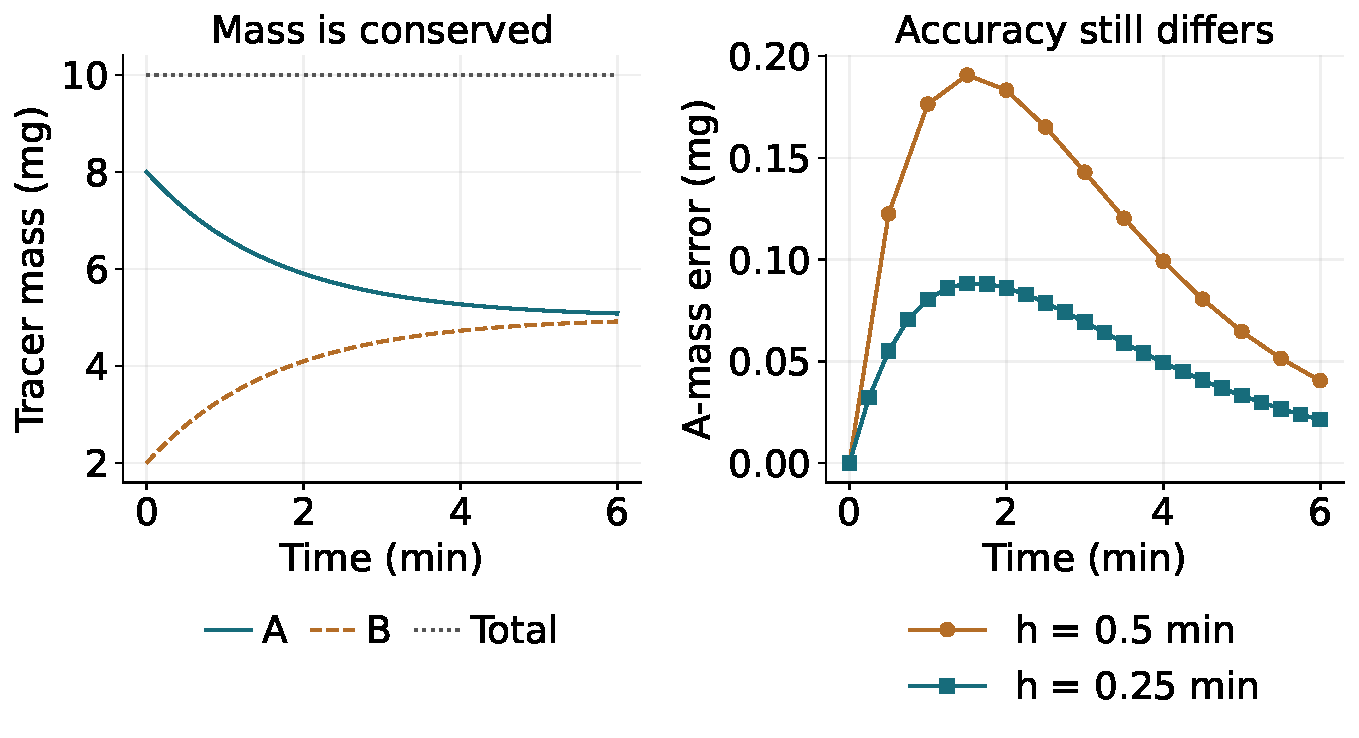
\includegraphics[width=.98\linewidth,height=.69\textheight,keepaspectratio]{exchange-and-error.pdf}\end{frame}
\renewcommand{\notestarget}{notes.pdf\#note-exact-solution}
\begin{frame}[t,fragile,label=slide-matrix-eigenmodes]{Matrix eigenmodes}
\[
\dot m=k\begin{pmatrix}-1&1\\1&-1\end{pmatrix}m.
\]
\pause{}
Eigenvectors $(1,1)^{\mathsf T}$ and $(1,-1)^{\mathsf T}$ have eigenvalues $0$ and $-2k$.
\end{frame}
\renewcommand{\notestarget}{notes.pdf\#note-euler-stability-and-positivity}
\begin{frame}[t,fragile,label=slide-euler-stability-and-positivity]{Euler stability and positivity}
\[
\begin{pmatrix}m_A^{n+1}\\m_B^{n+1}\end{pmatrix}
=\begin{pmatrix}1-kh&kh\\kh&1-kh\end{pmatrix}
\begin{pmatrix}m_A^n\\m_B^n\end{pmatrix}.
\]
\pause{}
Nonnegative coefficients require $0\leq kh\leq1$.
\end{frame}
\renewcommand{\notestarget}{notes.pdf\#note-euler-stability-and-positivity}
\begin{frame}[t,fragile,label=slide-the-difference-mode-multiplier]{The difference-mode multiplier}
\[
d_{n+1}=(1-2kh)d_n.
\]
\pause{}
Decay requires $0<kh<1$. Monotone decay requires $0<kh\leq1/2$. A conserved total can coexist with an inaccurate or oscillating state.
\end{frame}
\renewcommand{\notestarget}{notes.pdf\#note-step-refinement}
\begin{frame}[t,fragile,label=slide-step-refinement]{Step refinement}
\[
\epsilon_M=\max_n|m_A^n+m_B^n-10|,
\]
\pause{}
\[
E(h)=\max_n\|m^n-m(t_n)\|_2.
\]
For Euler, $E(h)=O(h)$ under ordinary smoothness assumptions.
\end{frame}
\renewcommand{\notestarget}{notes.pdf\#note-estimating-the-exchange-coefficient}
\begin{frame}[label=slide-parameter-evidence-figure]{Parameter evidence}
\centering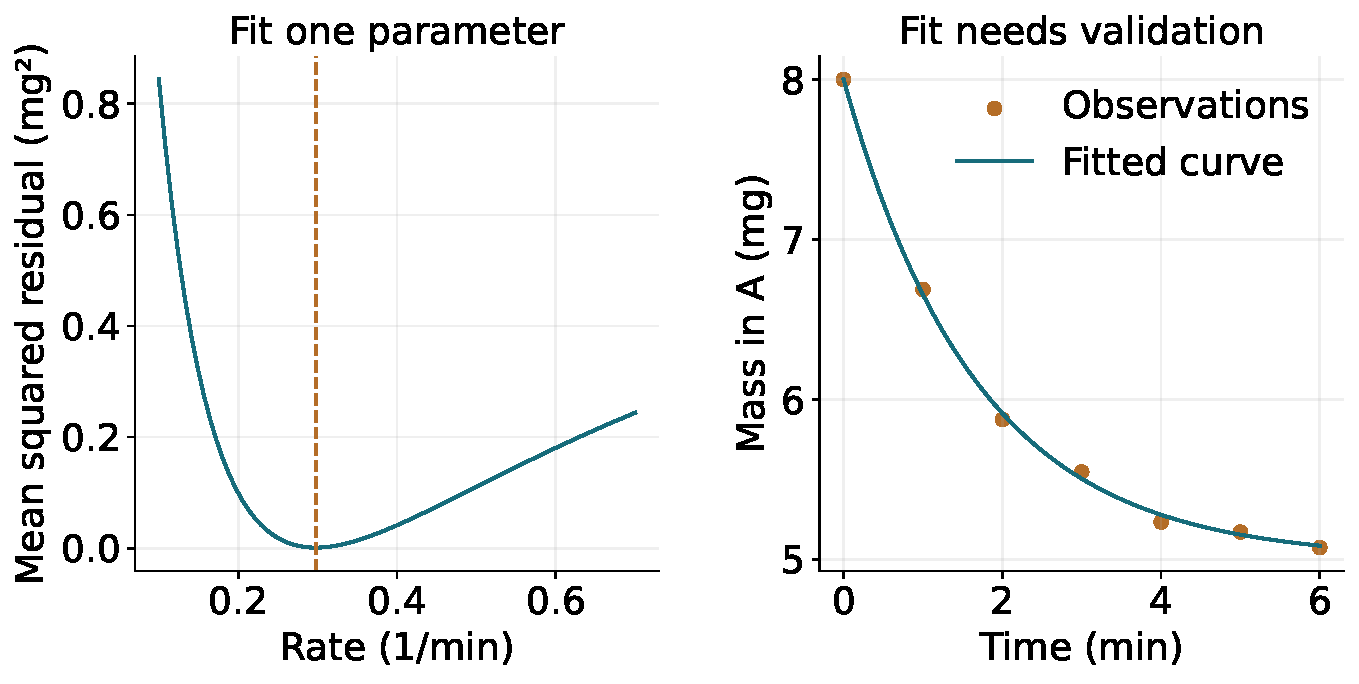
\includegraphics[width=.98\linewidth,height=.69\textheight,keepaspectratio]{parameter-evidence.pdf}\end{frame}
\renewcommand{\notestarget}{notes.pdf\#note-step-refinement}
\begin{frame}[t,fragile,label=slide-a-local-truncation-calculation]{A local truncation calculation}
\[
e^{-2kh}=1-2kh+2k^2h^2+O(h^3).
\]
\pause{}
Euler retains only the first two terms. The one-step difference is $O(h^2)$ and the accumulated fixed-time error is $O(h)$.
\end{frame}
\renewcommand{\notestarget}{notes.pdf\#note-estimating-the-exchange-coefficient}
\begin{frame}[t,fragile,label=slide-estimating-the-exchange-coefficient]{Estimating the exchange coefficient}
\[
J(k)=\sum_i[5+3e^{-2kt_i}-y_i]^2,\qquad k>0.
\]
\pause{}
\[
\partial_k m_A(t;k)=-6te^{-2kt}.
\]
\end{frame}
\renewcommand{\notestarget}{notes.pdf\#note-estimating-the-exchange-coefficient}
\begin{frame}[t,fragile,label=slide-informative-observation-times]{Informative observation times}
The initial measurement carries no sensitivity to $k$ when the initial state is fixed. Late measurements approach $5$ mg for every positive $k$.
\pause{}
The magnitude $te^{-2kt}$ is largest at $t=1/(2k)$.
\end{frame}
\end{document}
